\section{Evaluation}\label{sec:eval}

We first evaluate the graph using CLI commands, then deploy it through an
Apache Jena Fuseki SPARQL endpoint for a qualitative evaluation, because
Fuseki does not enable an OWL reasoner by default for the reasoning queries
used here.

The knowledge graph is evaluated through representative SPARQL queries
designed to demonstrate increasing expressiveness. The query collection is
organized into four categories: basic retrieval, structured filtering and
aggregation, reasoning-based queries, and cross-knowledge-graph queries.
Results below are trimmed to a compact representative
sample where the original query returns more records.

\subsection{Basic retrieval}

The first category tests direct access to resources and their descriptive
properties. The question asked in this example is: \emph{Which movies are
present in the knowledge graph?} The SPARQL pattern in
Table~\ref{tab:sparql-basic} retrieves movie names and local identifiers
without requiring joins beyond the movie type and name properties.
Table~\ref{tab:eval-basic} shows the first five returned records. These
results demonstrate that the graph can provide a simple catalogue view while
preserving stable resource identifiers for subsequent queries.

\begin{table}[!htbp]
    \centering
    \caption{SPARQL query for basic movie retrieval.}
    \label{tab:sparql-basic}
    \small
    \begin{tabular}{p{0.94\linewidth}}
        \toprule
        \texttt{SELECT DISTINCT ?movie\_id ?movie\_name} \newline
        \texttt{WHERE \{} \newline
        \texttt{\quad ?movie\_id a schema:Movie ;} \newline
        \texttt{\quad\quad schema:name ?movie\_name .} \newline
        \texttt{\}} \newline
        \texttt{LIMIT 20} \\
        \bottomrule
    \end{tabular}
\end{table}

\begin{table}[!htbp]
    \centering
    \caption{Representative results for basic movie retrieval.}
    \label{tab:eval-basic}
    \small
    \begin{tabular}{p{0.55\linewidth}p{0.35\linewidth}}
        \toprule
        \textbf{Movie} & \textbf{Local resource} \\
        \midrule
        Hope & \texttt{movie/1058424} \\
        Supergirl & \texttt{movie/1081003} \\
        Backrooms & \texttt{movie/1083381} \\
        Zootopia 2 & \texttt{movie/1084242} \\
        Toy Story 5 & \texttt{movie/1084244} \\
        \bottomrule
    \end{tabular}
\end{table}

\subsection{Structured filtering and aggregation}

The second category combines several graph patterns with filtering and
ordering. The question asked here is: \emph{Which are the highest-rated
Action movies released since 2020 that starred Tom Holland?} The SPARQL
pattern in Table~\ref{tab:sparql-structured} selects movies that satisfy
these conditions and orders them by rating value. Table~\ref{tab:eval-structured}
reports all three matching results in the generated dataset. Unlike the
basic retrieval query, this query traverses movie--genre, movie--role--actor, and
movie--rating relationships simultaneously, while also applying date and
value conditions.

\begin{table}[!htbp]
    \centering
    \caption{SPARQL query for multi-condition filtering and ranking.}
    \label{tab:sparql-structured}
    \small
    \begin{tabular}{p{0.94\linewidth}}
        \toprule
        \texttt{SELECT ?movie\_name ?genre ?date ?actor\_name ?rating\_value} \newline
        \texttt{WHERE \{} \newline
        \texttt{\quad ?id a schema:Movie ; schema:name ?movie\_name ;} \newline
        \texttt{\quad\quad schema:datePublished ?date ; schema:genre ?g ;} \newline
        \texttt{\quad\quad schema:actor ?a ; schema:aggregateRating ?rating .} \newline
        \texttt{\quad ?g schema:name "Action" .} \newline
        \texttt{\quad ?a schema:actor ?actor\_id .} \newline
        \texttt{\quad ?actor\_id schema:name "Tom Holland" .} \newline
        \texttt{\quad ?rating schema:ratingValue ?rating\_value .} \newline
        \texttt{\quad FILTER (?date >= "2020-01-01"\string^\string^xsd:date)} \newline
        \texttt{\}} \newline
        \texttt{ORDER BY DESC(?rating\_value)} \\
        \bottomrule
    \end{tabular}
\end{table}

\begin{table}[!htbp]
    \centering
    \caption{Results for multi-condition filtering and ranking.}
    \label{tab:eval-structured}
    \small
    \begin{tabular}{p{0.34\linewidth}p{0.16\linewidth}p{0.18\linewidth}p{0.15\linewidth}}
        \toprule
        \textbf{Movie} & \textbf{Year} & \textbf{Rating} & \textbf{Actor} \\
        \midrule
        The Odyssey & 2026 & 8.000 & Tom Holland \\
        Spider-Man: No Way Home & 2021 & 7.947 & Tom Holland \\
        Spider-Man: Brand New Day & 2026 & 7.860 & Tom Holland \\
        \bottomrule
    \end{tabular}
\end{table}

Table~\ref{tab:eval-structured} shows that the same graph can support
selection, joins, aggregation-ready rating values, and ranking in one
query. The result is therefore more expressive than a flat lookup because
the answer depends on several connected entity types and constraints.

\subsection{Reasoning-based queries}

The third category evaluates facts that are derived from the OWL ontology
rather than stored as direct movie attributes. The question is: \emph{Which
country is the production company of Avengers: Endgame from?} The SPARQL
pattern in Table~\ref{tab:sparql-reasoning} follows the inferred property
connecting the movie to its production country. OWL-RL reasoning is enabled
before query execution. The result in
Table~\ref{tab:eval-reasoning} identifies the United States of America,
although the query does not directly use the movie's country-of-origin
property.

\begin{table}[!htbp]
    \centering
    \caption{SPARQL query using an inferred production-country relation.}
    \label{tab:sparql-reasoning}
    \small
    \begin{tabular}{p{0.94\linewidth}}
        \toprule
        \texttt{SELECT ?country ?name} \newline
        \texttt{WHERE \{} \newline
        \texttt{\quad <https://example.org/movie/299534>} \newline
        \texttt{\quad\quad kg:productionCountry ?country .} \newline
        \texttt{\quad ?country schema:name ?name .} \newline
        \texttt{\}} \newline
        \texttt{ORDER BY ?name} \\
        \bottomrule
    \end{tabular}
\end{table}

\begin{table}[!htbp]
    \centering
    \caption{Result of an OWL-RL reasoning-based query.}
    \label{tab:eval-reasoning}
    \small
    \begin{tabular}{p{0.43\linewidth}p{0.43\linewidth}}
        \toprule
        \textbf{Movie} & \textbf{Inferred production country} \\
        \midrule
        Avengers: Endgame & United States of America \\
        \bottomrule
    \end{tabular}
\end{table}

Table~\ref{tab:eval-reasoning} illustrates the role of the ontology in
query answering. Without the property-chain inference, the requested
movie--country relationship would not be available through the same query
pattern. This category consequently demonstrates semantic enrichment
rather than only the retrieval of explicitly asserted triples.

\subsection{Cross-knowledge-graph queries}

The final category uses the \texttt{owl:sameAs} links to retrieve additional
information from an external knowledge graph. The question is: \emph{What
additional information about The Odyssey can be retrieved from DBpedia?}
The SPARQL pattern in Table~\ref{tab:sparql-external} follows the local
\texttt{owl:sameAs} link and retrieves properties of the external resource.
Since the complete external description contains many properties,
Table~\ref{tab:eval-external} shows selected results that complement the
local graph, including the film type, director, production company, budget,
and a starring actor.

\begin{table}[!htbp]
    \centering
    \caption{SPARQL query for retrieving linked external information.}
    \label{tab:sparql-external}
    \small
    \begin{tabular}{p{0.94\linewidth}}
        \toprule
        \texttt{SELECT ?p ?o} \newline
        \texttt{WHERE \{} \newline
        \texttt{\quad <https://example.org/movie/1368337>} \newline
        \texttt{\quad\quad owl:sameAs ?remote\_entity .} \newline
        \texttt{\quad ?remote\_entity ?p ?o .} \newline
        \texttt{\}} \\
        \bottomrule
    \end{tabular}
\end{table}

\begin{table}[!htbp]
    \centering
    \caption{Selected information retrieved from DBpedia for ``The Odyssey''.}
    \label{tab:eval-external}
    \small
    \begin{tabular}{p{0.36\linewidth}p{0.54\linewidth}}
        \toprule
        \textbf{Property} & \textbf{Retrieved value} \\
        \midrule
        Type & \texttt{dbpedia-ontology:Film} \\
        Director & Christopher Nolan \\
        Production company & Universal Pictures \\
        Budget & 250,000,000 \\
        Starring actor & Tom Holland \\
        \bottomrule
    \end{tabular}
\end{table}

Table~\ref{tab:eval-external} demonstrates that the local graph can act as
an entry point to information not collected in the local movie snapshot.
The local resource supplies the identity link, while DBpedia contributes
additional descriptive properties such as budget and production credits.
Taken together, the four query categories show a progression from direct
lookup to graph traversal, inference, and linked-data integration. They
demonstrate the practical expressiveness of the constructed knowledge graph
without interpreting the difficulty labels as formal research metrics.

\subsection{Fuseki SPARQL endpoint}

Figure~\ref{fig:fuseki-endpoint} provides a qualitative view of the deployed
Fuseki interface. It shows a SPARQL query submitted to the local endpoint and
the returned triples displayed in tabular form, demonstrating that the
generated knowledge graph is accessible through a browser-based SPARQL
service after the CLI-based evaluation.

\begin{figure}[!htbp]
    \centering
    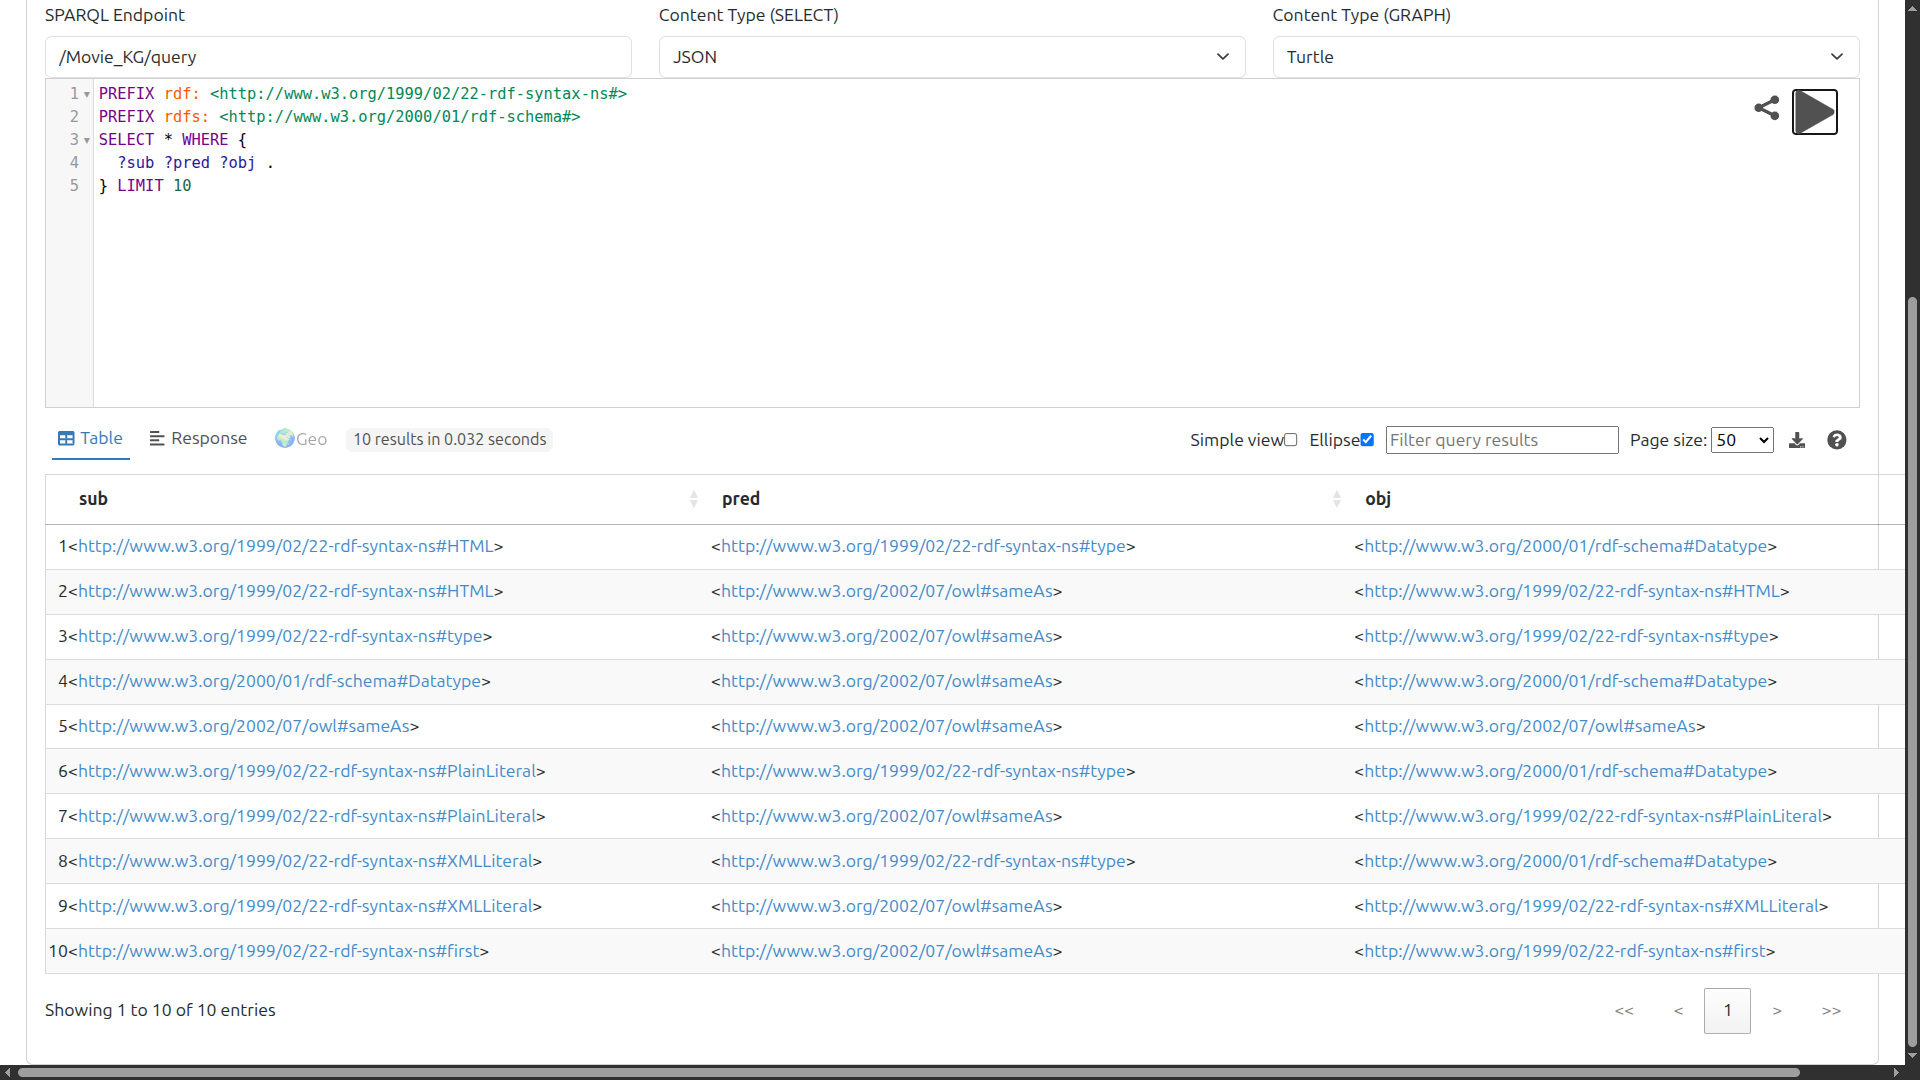
\includegraphics[width=\linewidth]{images/fuseki.png}
    \caption{Qualitative result from the Apache Jena Fuseki SPARQL endpoint.}
    \label{fig:fuseki-endpoint}
\end{figure}